\section{Stellensätze with denominators and Hilbert's 17th problem}

In this chapter, too, we deal with $n \in \N$ and indeterminates $X=(X_1,\ldots,X_n)$.

\subsection{Hilbert's 17th problem}

Non-negativity is not equivalent to SOS, but can one still certify non-negativity of polynomials algebraically in a different way? This already concerned Hilbert, who included the following problem on his famous list of the 23 problems from the year 1900: Is every non-negative polynomial in $\R[X]$ a sum of squares of rational functions?

Recall that we define the field $\R(X)$ of formal quotients $f / g$ with $f, g \in \R[X]$ and $g \ne 0$ with the standard multiplication and addition. 

Artin gave a complete positive solution of Hilbert's problem in 1927, and here we present a `modern version' of Artin's solution. It will turn out that as a byproduct we'll be able to derive a number of Stellensätze, which characterize non-negativity, positivity and equality to zero of a polynomial on a so-called basic closed semialgebraic set.

\subsection{Ordered fields}

We call a subset $P$ of a field $F$ a \emph{preordering} of the field $F$ if $P$ is closed under addition and multiplication, and every square is an element of $P$. That is $x+y \in P$ and $x y \in P$ for all $x, y \in P$ and $x^2 \in P$ for every $x \in F$. By $\sum F^2$ we denote the set of all sums of squares of elements of $F$. Clearly, one has $\sum F^2 \subseteq P$ for every preordering $P$ and $\sum F^2$ itself is a preordering.

If $F$ is a subset of a ring, we'll use the notation $\sum F^2$ for the set of all sums of squares of elements from $F$. For example, $\sum \R[X]^2$ is the set of all SOS-polynomials in variables $X$ with coefficients in $\R$ and $\sum \R(X)^2$ is the set of all sums of squares of rational functions in variables $X$.

We call a subset $P$ of $F$ an \emph{ordering} of $F$ if $P$ is closed under addition and multiplication and, furthermore, the equalities $P \cup (-P) = F$ and $P \cap (-P) = \{0\}$ hold. 

\begin{exercise}
\label{ex:ordering-preordering}
	Show that every ordering is a preordering. For this, it suffices to check that if $P$ is an ordering of the field $F$, then every square $x^2$ with $x \in F$ belongs to $P$.
\end{exercise} 
\begin{solution}
	One has either $1 \in P$ or $-1 \in P$. If we had $-1 \in P$, then we also had $(-1) (-1) = 1 \in P$, which is a contradiction. This shows that $1 \in P$. If $x \in F$ and $x \ne 0$, then we either have \blue{$x \in P$ or $-x \in P$}. In the former case $x^2 \in P$, because $x^2$ is a square of $x$ and in the latter case $x^2 \in P$, because $x^2$ is a square of $-x$. 
\end{solution}

Every ordering $P$ of $F$ defines a total-order relation $\le$ on $F$ given by $x \le y $ if and only if $y -x \in P$.  A field $F$ equipped with $P$ (and the total-order relation $\le$ arising from $P$) is called an ordered field. For an ordered field, one can also introduce $\ge, >$ and $<$ in a natural way. 

\begin{example}
	\label{ex:ordering:rational:functions}
	Let $n=1$ and consider the field $\R(X)$ of univariate rational functions. We order the subfield $\R$ of $\R(X)$ in a standard way ($\R_+$ is the standard ordering of $\R$). Let's order the whole $\R(X)$ by claiming that $X \ge r$ for every $r \in \R$. Once this is required, it is clear how the rest of $\R(X)$ gets ordered. For example, we have $X^2 \ge X$ and $X^3 \ge X$.
	\blue{Since $X \in P$ and $-1 \notin P$ (see Exercise~\ref{ex:ordering-preordering}), we cannot have $-1/X \in P$, and thus $1/X \in P$.
	Therefore, for every $r \in \R$ with $r > 0$, we have $r - 1/X = (rX-1) / X \in P$, which implies that $1/X < r$}. In this ordering $X$ is infinitely large, $X^2$ is even larger, $1/X$ is infinitely small positive, $1/X^2$ is even smaller etc. 
\end{example}

\begin{exercise}
	\label{exer:all:orderings:rational:functions}
	The field $\R(X)$ in the above example can be ordered in more than one way. 
	\begin{enumerate}[(a)]
		\item Try to find other orderings that extend the ordering of $\R$. 
		\item Can you describe all such orderings? 
	\end{enumerate}
\end{exercise}
\begin{solution}
	(a): Just by interchanging the roles of $X$ and $1/X$, we get another ordering. In this ordering, $1/X$ is infinitely large. One can also require $-X$ to be infinitely large or $-1/X$ to be infinitely large. 
	
	(b): Yet another general possibility (that covers the case of $1/X$ or $-1/X$ being infinitely large) is to fix a number $a \in \R$ and require $X-a$ to be infinitely small positive or infinitely small negative. It is not very hard to convince oneself that the above suggestions cover all possible orderings. In fact, $\R$ is already ordered, and $X$ should occupy some place with respect to the real numbers. We can put it either behind all real numbers or before all real numbers, or fix $a \in \R$ and put $X$ before $a$ or behind $a$ (infinitely close to $a$). 
\end{solution}

We call a field $R$ \emph{real closed} if $R$ is not algebraically closed but \blue{$R(\sqrt{-1})$} is an algebraically closed field. That is, in $R$ we only miss an imaginary unit for representing the roots of polynomial equations. The abstract field \blue{$R(\sqrt{-1})$} is in the same relation to the abstract field $R$ as the field $\mathbb{C}$ of complex numbers to the field $\R$ of real numbers. 

\begin{exercise}
Show the following. For a real closed field $R$, the set  $\sum R^2$ is the unique ordering of $R$. Even more specifically, an element of $R$ is non-negative \blue{with respect to any given ordering} if and only if it is a square $x^2$ with $x \in R$. 
\end{exercise}
\begin{solution}
	Let $i:= \sqrt{-1}$. Consider an arbitrary ordering of $R$ and let's denote the corresponding order relation (as usual) by $\le$.
%	If $a \in R \setminus \{0\}$ satisfies $a \ge 0$,
    \blue{For any $a \in R \setminus \{0\}$, }the equation $\lambda^2 = a$ has two roots in \blue{$R(i)$}. These roots are either of the form $\pm b$ with $b \in R \setminus \{0\}$ or of the form $\pm i b$ with $b \in R \setminus \{0\}$. In the first case $a = b^2$. In the second case $a = - b^2$. Since $b^2 \ge 0$, we see that in the former case $a \ge 0$ and in the latter case $a \le 0$. Thus, the whole $R$ gets decomposed into squares and `minus squares' (that intersect at the element $0$). This shows that squares are all the non-negative elements with respect to our ordering. 
\end{solution}

\begin{theorem}
	\label{thm:extending:to:real:closed}
	For every ordered field $F$ there exists a (unique) real closed extension~\blue{$R$ of~$F$}. This means $R$ is an extension of the field $F$, $R$ is a real closed field and the set of all elements in $R$ which are non-negative in $R$ and belong to $F$ is exactly the set of all elements of $F$ that are non-negative in $F$. 
\end{theorem}
\begin{proof}
	The proof is contained in \cite{Bochnak:Coste:Roy:1998} (one of the first chapters). 
\end{proof}

\subsection{Quantifier elimination and Tarski's transfer principle}

Let $R$ be a real closed field (for example, $R=\R$).  We start with some terminology
\begin{itemize}
	\item A \emph{boolean formula} is a formula based on and,or,not operations and involving boolean variables (true/false-variables).
	\item A \emph{quantifier-free formula} $F$ is obtained by plugging in relations of the form $f(X)=0, f(X)>0, f(X) \ge 0$ etc. for $f \in R[X]$ into a boolean formula. So, a quantifier-free formula depends on indeterminates. If the underlying polynomials have rational coefficients (that is $f \in \Q[X]$), we say that the formula has rational coefficients.
	\item A \emph{first-order formula} is a formula, in which some of the variables are quantified. It has the form 
	\[
		F(X):= \mathcal{Q}_1 Y_1 \ldots \mathcal{Q}_k Y_k \ \ G(X_1,\ldots,X_n,Y_1,\ldots,Y_k),
	\] where $G$ is a quantifier-free formula and $\mathcal{Q}_1,\ldots,\mathcal{Q}_k \in \{ \forall, \exists\}$ are quantifiers.
	\item Two formulas $F_1(X)$ and $F_2(X)$ are said to be \emph{equivalent} over $R$ if $F_1(x)=F_2(x) \ \blue{\in \{\texttt{true},\texttt{false}\} = \{0,1\}}$, for all $x \in R^n$. 
\end{itemize}


\begin{theorem}[Tarski-Seidenberg quantifier elimination] 
	\label{thm:tarski-seidenberg}
	Let $R$ be a real closed field. Let $F$ be a first-order formula with rational coefficients. Then there exists an algorithm that constructs a quantifier-free formula $G$ with rational coefficients equivalent to $F$. The algorithm depends only on $F$ and not on the choice of the underlying real closed field $R$. 
\end{theorem}
\begin{proof}[About the proof]
	The proof is not particularly hard but a bit long. It proceeds by induction, and one basic thing one should learn to do is counting real roots of a polynomial in an interval (to start the induction). A complete proof can be found in \cite[Thm.~1.4.6]{Bochnak:Coste:Roy:1998}. If abstraction is not your favorite activity, one can read the proof setting $R=\R$, but the point is that for every real closed field $R$ the proof works just the same, and this will turn out to be a \emph{crucial} observation when it comes to proving Stellensätze. 
\end{proof}

Sets defined by a first-order formula are called \emph{semialgebraic}.
These are precisely the sets of the form $\setcond{x \in R^n}{F(x)=0}$, where $F(X)$ is a first-order formula with free variables $X=(X_1,\ldots,X_n)$. Semialgebraic sets defined by a system of only non-strict resp.\ only strict polynomial inequalities are called \emph{basic closed} resp.\ \emph{basic open}.

\begin{exercise}
	Let $k,d \in \N$. 
	\begin{enumerate}[(a)]
		\item Is $\cS_+^k$ semialgebraic? Is it basic closed semialgebraic?
		\item Is $\intr(\cS_+^k)$ semialgebraic? Basic open semialgebraic?
		\item Is the set of all non-negative $n$-variate polynomials of degree at most $2d$ semialgebraic?
		\item Is the set of all positive $n$-variate polynomials of degree at most $2d$ semialgebraic?
	\end{enumerate}
\end{exercise}

\begin{remark}[Quantifier elimination algorithms]
	Currently, the best algorithms to perform quantifier elimination carry out the quantifier elimination procedure in $O((m d)^{O(n^{4 (t+1)})})$ arithmetic operations, where $m$ is the number of polynomials involved, $d$ \blue{is an upper bound on the degree of those polynomials}, and $t$ is the number of quantifier alternations. In particular, if there are no alternations (say, all the quantifiers are existential), the time bound is exponential. In principle, one can solve polynomial optimization problems using quantifier elimination in exponential time, \blue{so that POP is in EXP as mentioned in the introduction;} but no one would dare to do that on large problems. One reason for the running time being so high, is that in certain situations the output (quantifier-free formula equivalent to the given one) is exponentially large. 
\end{remark}

\begin{remark}[Fourier-Motzkin elimination]
	Fourier-Motzkin elimination is a special case of quantifier elimination occurring in the theory of polyhedra and linear programming. We have a system of affine linear inequalities of the form $f_1(x,y) \ge 0,\ldots,f_m(x,y) \ge 0$ in variables $x \in \R^n$ and $y \in \R$ and we want to write the condition that there exists \blue{a real number} $y$ satisfying $f_1(x,y) \ge 0,\ldots, f_m(x,y) \ge 0$ in terms of $x$-variables only. This is possible. \blue{Due to the linearity of the functions $f_i$}, the inequalities can be written in the form $y \le u_i(x)$, $y \ge l_j(x)$ and $g_k(x) \ge 0$ with $i \in I$, $j \in J$ and $k \in K$. That is, each inequality either provides an upper bound on $y$, or a lower bound on $y$, or is independent of $y$. Now, the existence of $y$ can be written as the system $\max_{j \in J} l_j(x) \le y \le \min_{i \in I} u_i(x)$, $g_k(x) \ge 0$ for every $k$. The system can be reformulated without any use of $y$ as $l_j(x) \le u_i(x), g_k(x) \ge 0$ for all $i \in I, j \in J, k \in K$. One can see that out of $m$ original inequalities one gets up to $\Theta(m^2)$ inequalities after elimination. There exist examples that show that this cannot be avoided. The situation in general quantifier elimination is pretty similar. 
\end{remark}

Just to get a feeling how quantifier elimination can be carried out, let us consider a particular example. 

\begin{exercise}
	Compute a quantifier-free formula equivalent to 
	\[
		F(p,q) := \exists x \ \bigl[ \ -1 \le x \le 1 \  \text{and} \ x^2 + p x + q = 0  \ \bigr].
	\]
	Draw a sketch of the respective semialgebraic set $S:= \setcond{(p,q) \in \R^2}{F(p,q) =0}$. 
\end{exercise}
\begin{solution}
	The condition $F(p,q)$ just tells us that the quadratic polynomial $f(X):=X^2 + p X + q$ given by coefficients $p$ and $q$ has a root in the segment $[-1,1]$. Let's figure out how we could characterize this condition in $p$ and $q$ directly, without any use of quantifiers. If the signs of $f$ at the endpoints of $[-1,1]$ are different, we'll get a root in $[-1,1]$ (by the intermediate value theorem from analysis). So, we'll have a root if $f(-1) \ge 0$ and \blue{$f(1) \le 0$}, or if $f(-1) \le 0$ and $f(1) \ge 0$. If $f(-1) < 0$ and $f(1) < 0$, we'll have no roots in $[-1,1]$, because $f$ is convex. So, we are left with the case $f(-1) \ge 0, f(1) \ge 0$. Note that the global \blue{minimum} of $f$ is attained at $x = -p/2$. Thus, if $x = -p/2$ is in $[-1,1]$ and $f(-p/2) \le 0$, then $f$ has a root in $[-1,1]$. 
	
	To sum up, if at least one of the following cases occurs, $f$ has a root in $[-1,1]$:
	\begin{enumerate}[(a)]
		\item $f(-1) \le 0, f(1) \ge 0$ or 
		\item $f(-1) \ge 0, f(1) \le 0$ or 
		\item $f(-1) \ge 0, f(1) \ge 0$, $-1 \le -p/2 \le 1$, $f(-p/2) \le 0$.
	\end{enumerate}
	Conversely, if neither of the above cases occurs, we must have $f(-1)<0, f(1) < 0$ or $f(-1) > 0, f(1) > 0$. In the former situation, $f$ has no roots in $[-1,1]$, which follows from convexity of $f$. In the latter situation, if $-p/2$ lies outside $[-1,1]$, then $f$ has no roots in $[-1,1]$ (because $f$ either grows or falls in $[-1,1]$ and remains strictly positive on the whole segment). If $-p/2 \in [-1,1]$, we have $f(-p/2) > 0$ (for, otherwise, the third condition would be fulfilled), which shows that $f$ is strictly positive on $\R$ and thus also on $[-1,1]$. Thus, we have characterized $F(p,q)$ by the above three conditions. In terms of $p$ and $q$ the conditions can be formulated as 
	\begin{enumerate}[(A)]
		\item $1 - p + q \le 0, 1 + p + q \ge 0$ or 
		\item $1 - p + q \ge 0, 1 + p + q \le 0$, or
		\item $1 - p+ q \ge 0, 1 + p + q \ge 0$, $-1 \le -p/2 \le 1$, $p^2 - 4 q \ge 0$. 
	\end{enumerate}
	Here is a picture of the semialgebraic set described by $F(p,q)$: 
	\begin{center}
		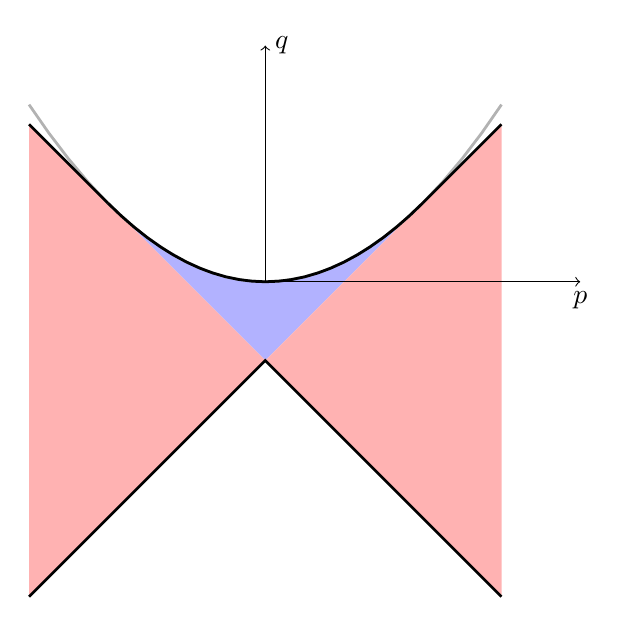
\begin{tikzpicture}
		\fill[blue!30!white,domain = -2:2] plot ({\x}, {\x*\x*0.25}) -- (0,-1); 
		\fill[red!30!white] (0,-1) -- (-3,2) -- (-3,-4) -- cycle;
		\fill[red!30!white] (0,-1) -- (3,2) -- (3,-4) -- cycle;
		
		\draw[black!30!white,domain = -3:3,line width = 1pt,line width = 1pt] plot ({\x}, {\x*\x*0.25});
		\draw[domain = -2:2,line width = 1pt,line width = 1pt] plot ({\x}, {\x*\x*0.25});
		\draw[line width=1pt] (-3,-4) -- (0,-1) -- (3,-4);
		\draw[line width=1pt] (2,1) -- (3,2);
		\draw[line width=1pt] (-2,1) -- (-3,2);
		
		\draw[<->] (0,3) node[right]{$q$} -- (0,0) -- (4,0) node[below]{$p$};
		\end{tikzpicture}
	\end{center}
\end{solution}

	This exercise illustrates the following situation. Assume that you are optimizing a function $g(p,q)$ subject to constraints $-1 \le x \le 1$ and $x^2 + p x + q =0$. Even though, it looks as if your feasible set is nice (it is just a piece of a surface described by a simple equation $x^2 + p x + q =0$), projecting out $x$ and writing your constraints without $x$, you see that you are optimizing $g$ over a weird semialgebraic subset of $\R^2$ (which is not basic: it cannot be described by a system of polynomial inequalities). This is in contrast to the situation in linear optimization. In linear optimization, a projection of a polyhedron is a polyhedron again. This exercise shows that a projection of a basic semialgebraic set is not necessarily basic. 

As a consequence of \blue{the Tarski-Seidenberg theorem}, we obtain the following crucial corollary. It says that whenever a first-order formula over $\R$ is satisfiable over a bigger real closed field $R$, then it is also satisfiable over our original smaller field $\R$. 

\begin{corollary}[Tarski's transfer principle]  
	\label{cor:tarski}
	Let $R$ be a real ordered field, \blue{that is,} an ordered extension of the field $\R$. Let $F(X)$ be a first-order formula with coefficients in $\R$. If there exists an $x^\ast \in R^n$ such that $F(x^\ast)$ is fulfilled, then there exists also an $x' \in \R^n$ such that $F(x')$ is fulfilled. 
\end{corollary}
\begin{proof}
	The proof is borrowed from \cite[Cor.~1.4.7]{Bochnak:Coste:Roy:1998}. \blue{In view of Theorem~\ref{thm:extending:to:real:closed}}, it is known that the real ordered field \blue{$R$} can be extended to a real closed field \blue{$R'$} (see \cite{Bochnak:Coste:Roy:1998}).
	\blue{We work over the larger field $R'$.}
%	So, without loss of generality we assume that $R$ is real closed. 
	
	Let $Y=(Y_1,\ldots,Y_k)$ be the quantified variables used in $F(X)$. 
	Each polynomial $f \in \R[X,Y]$ involved in $F(X)$ can be written as $f(X,Y) = g(X,Y,a)$, where $a \in \R^m$
%	is independent of $f$
	and where $g \in \Q[X,Y,Z]$ (a polynomial with rational coefficients) and $Z=(Z_1,\ldots,Z_m)$ are additional indeterminates. For example, if $f(X,Y) = \sqrt{2} X^2 + \sqrt{3} (X-Y) + \sqrt{2} Y^2$ we can introduce $g(X,Y,Z_1,Z_2) = Z_1 X^2 + Z_2 (X-Y) + Z_1 Y^2 \in \Q[X,Y,Z_1,Z_2]$ with $f(X,Y,a) = f(X,Y)$ for $a=(\sqrt{2},\sqrt{3})$.
		That is, we put all the real coefficients of all the polynomials involved in $F(X)$ into a vector $a$.
		
		This gives rise to a first-order formula $G(X,Z)$ such that $G(X,a) = F(X)$. By Tarski-Seidenberg \blue{(Theorem~\ref{thm:tarski-seidenberg})}, $\exists X : G(X,Z)$ can be turned into a quantifier-free formula. So, there exists a quantifier-free formula $H(Z)$ with rational coefficients equivalent to $\exists X : G(X,Z)$ over every real closed field. We plug in $Z=a$ and see that $\exists X : G(X,a)$ is equivalent to $H(a)$, where $H(a)$ is independent of $X$ and so $H(a)$ is either true or false. By assumption $\exists X : G(X,a) = \exists X : F(X)$ is true over~$R$, \blue{and hence true over $R'$}. So, $H(a)$ is true and so $\exists X : G(X,a) = \exists X : F(X)$ is true over every real closed field containing $\R$ including $\R$ itself. This gives the assertion. 
\end{proof}

\subsection{Solution of Hilbert's 17th problem}

\begin{lemma}[Serre 1947]
	\label{lem:Serre}
%	Let $F$ be field of zero characteristic (this means that $\underbrace{1+ \cdots + 1}_k \ne 0$ in $F$ for every $k \in \N$).
	\blue{Let $F$ be field of characteristic not equal to two (this means that $1 + 1 \ne 0$ in $F$).}
	Let $T$ be a preordering of $F$ and let $f \in F \setminus T$.
	\blue{Every} inclusion-maximal preordering $P$ with the properties $T \subseteq P$ and $f \not\in P$ is an ordering. 
\end{lemma}

\begin{proof}
	Note that the existence of $P$ follows from Zorn's lemma (and is by this based on the axiom of choice).
	\blue{The partially ordered set to be considered is
	\[
    \mathcal{P} := \left\{ P \subseteq F : T \subseteq P, f \notin P \textrm{ and } P \textrm{ is a preordering}\right\}.
	\]
    If $\mathcal{C} \subseteq \mathcal{P}$ is a chain, then the set $I = \bigcup_{P \in \mathcal{C}} P$ is an upper bound on~$\mathcal{C}$ in~$\mathcal{P}$.
	}
	
	We recall that a preordering is a set closed under addition, multiplication and taking squares. We also shortly mention that a preordering is closed under divisions, too. If both $a$ and $b$ are in the preordering and $b$ is not zero, then $a/b = a b (1/b)^2$ and so, we see that immediately.
	
	We first observe that $-1 \not\in P$. In fact, if we had $-1 \in P$, then $P$ is going to be the whole field $F$, which is a contradiction \blue{to the assumption that $f \notin P$}. To see this, it suffices to observe that every element of $F$ is a difference of two squares. Just use the simple identity $ 4 x = (1+x)^2 - (1-x)^2$ and divide it by four (division by four requires $1+1 \ne 0$ in $F$ -- this is the reason of having the assumption on the characteristic of the field $F$). All squares are in the preordering just by definition. If $-1$ is in $P$, then also the minus squares are in the preordering. But then also the differences of the squares are in the preordering and we get $P=F$, which contradicts $f \not\in P$. 
	
	
	We also note that $-f \in P$. If we had $-f \not \in P$, we would get that the set $P - f P$ containing both $P$ and $-f$ is a preordering, \blue{and thus $P$ is not maximal}. In fact, $P - f P$ is closed under addition, because $P$ is closed under addition, $P-f P$ contains all squares, because $P$ contains all squares and $P- f P$ is closed under multiplication, which can be seen by expanding the brackets in $(P -f P)(P - fP)$ and using the fact that $P$ is a preordering. 
	
	Furthermore, since $P$ does not contain $f$, also the set $P - fP$ does not contain $f$. For if $f \in P - fP$, then we had $f = a - f b$ with $a, b \in P$, which gives $(1+b) f = a$. We have $b+1 \ne 0$, since otherwise $-1 = b \in P$ would be an element of $P$. Consequently, $ f= a / (1+b) \in P$, which is a contradiction.
	
	Furthermore, we observe that for every $g \in F$, one has $g \in P$ or $-g \in P$, which means $P \cup (-P) = F$. 
	If, say, $g \not \in P$, we'll show that $-g \in P$. Consider the set $P + g P$. As above, $P + g P$ is a preordering containing $P$, and the containment is proper because $g \in P+ gP$ and $g \not\in P$. By the inclusion-maximality of $P$ under the property $f \not\in P$, we must have $f \in P + gP$, which means that $f = a + g b$ holds for some $a,b \in P$. Then $ - b g = a + (-f) \in P$, because $a \in P$ and we have seen that $-f$ belongs to $P$, too. One cannot have $a - f= 0 $, since otherwise $f = a \in P$. This implies $g b = f -a  \ne 0$. \blue{As a field has no zero-divisors, this implies that} $b \ne 0$, and by this $-g = (a-f) / b \in P$. 
	
	It remains to show that $P \cap (-P) = \{0\}$ holds. Let $g \in P \cap (-P)$, that is $g, - g \in P$. Then $g =0$, for otherwise, we had $-1 = g (-g) (1/g)^2 \in P$, which contradicts $-1 \not\in P$, which we have derived above. 
\end{proof}

\begin{theorem}[Artin 1927] Let $f \in \R[X]$ be a non-negative polynomial. Then $f \in \sum \R(X)^2$ (that is, $f$ is a sum of squares of rational functions). 
\end{theorem}
\begin{proof}
	Assume to the contrary that $f \not \in \sum \R(X)^2$. Applying Lemma~\ref{lem:Serre} to the preordering $\sum \R(X)^2$ of $\R(X)$, we see that there exists an ordering $P$ on $\R(X)$ with respect to which $f$ is negative. We fix $R := \R(X)$ and endow $R$ with the ordering $P$ (this can be viewed as follows: $P$ is a kind of evaluation of rational functions at an `abstract point' and by construction $f$ is strictly negative at this abstract point). By construction, there exists $(x_1,\ldots,x_n) \in R^n$ such that $f(x_1,\ldots,x_n) < 0$. Indeed $X_1,\ldots,X_n$ are rational functions and hence elements of $R$, and so $f(x_1,\ldots,x_n) < 0$ holds for $(x_1,\ldots,x_n) \in R^n$ with $x_1=X_1,\ldots,x_n=X_n$. Since $R$ is a field extending $\R$ and since the coefficients of the polynomial $f$ are in $\R$, Tarski's principle  shows that there also exists $(x_1,\ldots,x_n)$ belonging to $\R^n$ such that $f(x_1,\ldots,x_n) < 0$. This contradicts the non-negativity of $f$. Consequently, $f \in \sum \R(X)^2$. 
\end{proof}

\begin{remark}
The previous proof is not constructive, so it does not provide a method to write a non-negative polynomial as a sum of squares of rational functions. E.g., from the proof, it is not clear \emph{how} the Motzkin polynomial (or other non-SOS-polynomials) can be represented as a sum of squares of rational functions. 

\blue{However, there is a way to often find such representations based on the following idea: If you want to write a non-negative polynomial $f \in \R[X]$ as
\[
f = \left(\frac{h_1}{g_1}\right)^2 + \ldots + \left(\frac{h_r}{g_r}\right)^2
\]
for some $h_i,g_i \in \R[X]$, then one could try to go for a common denominator~$q$ and represent $q \cdot f$ as a sum of squares of polynomials.
For instance, if~$f$ is the Motzkin polynomial, then one finds
\begin{align*}
(1 + X^2 + Y^2) \cdot f &= (X^2 - Y)^2 + (XY^2 - X)^2 + (X^2Y^2 - 1)^2 + \frac14 (XY^3 - X^3Y)^2\\
&\phantom{=} + \frac34 (XY^3 + X^3Y - 2XY)^2.
\end{align*}
Hence, multiplying once more with $(1+X^2+Y^2)$ results in a representation for $f \in \sum \R(X,Y)^2$.}

\blue{This works almost in all cases in view of a result of Reznick (1995); see~\cite{reznick1995uniform}: If $f \in \R[X]$ is such that $\inf_{x \in \R^n} f(x) > 0$, then there is an $r \in \N_0$ such that $(1 + X_1^2 + \ldots + X_n^2)^r \cdot f$ is SOS.
}
\end{remark}

\begin{remark}
	It is known that $2^n$ squares suffice. For $n=1$, we have seen this in our proof. The case $n=2$ is due to Hilbert (1893). The general case is due to Pfister (1965); see \cite{Bochnak:Coste:Roy:1998}. 
\end{remark}

\subsection{An algebraic certificate of non-negativity}

Now, let's consider a more general setting, in which we want to certify whether a polynomial $f$ is positive or non-negative on a basic closed semi-algebraic set $K$. The solution of Hilbert's 17th problem gives a certificate for $K=\R^n$ and, using similar principles, we can also do the case of a more general $K$. 

Given $s$ polynomials $g=(g_1,\ldots,g_s) \in \R[X]^s$, we introduce the basic closed set 
\[
	\{g \ge 0\} := \setcond{x \in \R^n}{g(x) \ge 0}.
\]
We'll also use the longer notation
\[
	\{g_1 \ge 0,\ldots, g_s \ge 0\} := \setcond{ x \in\R^n}{g_1(x) \ge 0,\ldots,g_s(x) \ge 0},
\]
and we'll use an analogous notation for strict inequalities and equalities. With $g$ we also associate
the so-called preordering generated by $g$, defined as
\begin{align*}
	\cP(g) & := \cP(g_1,\ldots,g_s) 
	\\ & := \setcond{\sum_{e:=(e_1,\ldots,e_s) \in \{0,1\}^s} \sigma_e g_1^{e_1} \ldots g_s^{e_s} }{ \sigma_e \ \text{is SOS} \ \text{for every} \ e \in \{0,1\}^s}.
\end{align*}
For example, for $s=2$, $\cP(g_1,g_2)$ consists of polynomials $\sigma_{0,0} + \sigma_{1,0} g_1 + \sigma_{0,1} g_2 + \sigma_{1,1} g_1 g_2$, where $\sigma_{0,0}, \sigma_{1,0}, \sigma_{1,0}, \sigma_{1,1}$ are SOS. 
\blue{Also, $\cP(0) = \sum \R[X]^2$.}

Clearly, $\cP(g)$ is indeed a preordering and it is the inclusion-minimal preordering containing all the polynomials $g_1,\ldots,g_s$. Each $f \in \cP(g)$ is non-negative on $\{g \ge 0\}$. Furthermore, we can recover $\{g \ge 0\}$ from $\cP(g)$ since we obviously have 
\[
	\{g \ge 0\} = \setcond{x \in \R^n}{f(x) \ge 0 \ \text{for all} \ f \in \cP(g)}.
\]
The latter equality allows us to view $\cP(g)$ as a kind of dual object associated to the semi-algebraic set $\{g \ge 0\}$. 

While the condition that $f \ge 0$ on $\{g \ge 0\}$ is a `geometric' non-negativity condition ($f$ non-negative on a semi-algebraic) set, $f \in \cP(g)$ is a sort of `algebraic' non-negativity condition. Though it is not true that the two conditions are equivalent, there is a strong relationship and, for understanding the ideas of the following proofs, it is nice to keep in mind the analogy between the two notions. 

We also introduce the set 
\[
	\cP^0(g):= \cP(g) \cap (-\cP(g)).
\]

\begin{itemize}
	\item A representation of $f$ as an element of $\cP(g)$ provides an algebraic evidence for $f \ge 0$ on $\{g \ge 0\}$. 
	\item A representation of $f$ as an element of $\cP^0(g)$ provides an algebraic evidence for $f = 0$ on $\{g \ge 0\}$. 
\end{itemize}

So, it is nice to think of $f \in \cP(g)$ and $f \in \cP^0(g)$ as some kind of `$\ge 0$' and `$=0$' conditions. 

%Sometimes we'll work with sets $F$ that are larger than $\R$, and the we'll use subscript $F$, like $\cP_F(g)$ We will also use notation 

%\[
%	\{ g \ge 0\}_F := \setcond{x \in F^n}{g(x) \ge 0}
%\] 
%for ordered fields extending $\R$ and we'll use the notation like

%\[
%	\cP_F(g) := \setcond{ \sum_{e =(e_1,\ldots,e_s) \in \{0,1\}^s} \sigma_e g_1^{e_1} \cdots g_s^{e_s}}{\sigma_e \in \sum F[X] \ \forall e}
%\]
%where $F$ is a field or ring. 

We recall that an ideal $I$ in a commutative ring $(R,+,\cdot)$ is an additive subgroup of $R$ with the property $I R \subseteq I$. 

\begin{lemma}
	\label{lem:ideals}
	Let $n \in \N$. Let $g=(g_1,\ldots,g_s) \in \R[X]^s$, let $P:=\cP(g)$ and $I:=\cP^0(g)$. Then, the following hold: 
	\begin{enumerate}[(a)]
		\item \label{I:ideal} $I$ is an ideal in $\R[X]$.
		\item \label{I:proper} If $I$ is proper (that is $I \ne \R[X]$), then $-1 \not\in P$ (analogy: if there is an element not equal to zero `in the abstract sense', the constants like $-1$ are not non-negative `in the abstract sense').
		\item \label{sum:non-neg:zero} If $p, q \in P$ and $p+q \in I$, then $p, q \in I$ (analogy: if the sum of non-negative elements is zero, then all the summands are zero). 
	\end{enumerate}
\end{lemma}
\begin{proof}
 \eqref{I:ideal}: Since $P$ is closed under addition, $I$ too is closed under addition. Since $0 \in P$, we have $0 \in I$ and it is clear that $I + I = I$. For every $f \in I$ also $-f \in I$. So $(I,+)$ is a subgroup of $\R[X]$.
 
 Let $q \in I = P \cap (-P)$. As we did above, we use a formula telling us that every element of $\R[X]$ is a difference of two squares.
  For every $p \in \R[X]$, one has $ 4 p = (1+p)^2 - (1-p)^2$. Since $(1+p)^2 q \in P \cap (-P)$ and $(1-p)^2 q \in P \cap (-P)$, we conclude that $4 p q \in P \cap (-P)$.
 \blue{The latter holds since we just showed that $(I,+)$ is a group.}
  Dividing by $4$, we get $p q \in P \cap (-P)$.
%  Here is a bit more detailed explanation how we can get the conclusion: From $q \in P$ and $-q \in P$, we get $(1+p)^2 q \in P$ and $-(1-p)^2 q \in P$, respectively. This yields $(1+p)^2 q - (1-p)^2 q \in P$, meaning $4 p q \in P$. Dividing by~$4$, we get $p q \in P$. Completely analogously, we also get $p q \in -P$. 
 
 \eqref{I:proper}: If $-1 \in P$, then using $ 4 p = (1+p)^2 - (1-p)^2$, we conclude that $P = \R[X]$. Hence $I=P \cap (-P) = \R[X]$, which is a contradiction. 
 
 \eqref{sum:non-neg:zero}:
% Since, $p,q \in P$, we have $p+q \in P$.
% So we just need to show $-p, -q \in P$. Indeed, showing this, we get $-(p+q) \in P$ and conclude $p+q \in P \cap (-P) = I$.
 \blue{Since $p+q \in I$, we have $-p - q \in P$. So $-p \in q + P \subseteq P$ and $-q  \in p +P \subseteq P$, because $p,q \in P$ and $P$ is closed under addition.
 Hence, $p,q \in P \cap (-P) = I$.}
\end{proof}

The ideal $\cP^0(g)$ should help us to certify the condition $f=0$ on $\{g \ge 0\}$. However, $\cP^0(g)$ may have an undesired property of being non-prime. Here is just a small example with $g=(g_1,g_2)$, $g_1=X_1 X_2, g_2 = -X_1 X_2$. In this case, the set $\{g \ge 0\} = \{X_1 X_2 = 0\}$ is just the union of two coordinate axes. The polynomial $X_1$ does not belong to $\cP(g)$, because $X_1$ is not non-negative on $\{g \ge 0\}$. Analogously, the polynomial $X_2$ does not belong to $\cP(g)$ because $X_2$ is not non-negative on $\{g \ge 0\}$. It is clear that the product $X_1 X_2$ belongs to $\cP^0(g)$. So, we conclude that neither $X_1$ nor $X_2$ belongs to $\cP^0(g)$ but their product $X_1 X_2$ does belong to $\cP^0(g)$. This shows that the ideal $\cP^0(g)$ is not prime. The reason of $\cP^0(g)$ being non-prime is the fact that the variety $\{X_1 X_2 = 0\}$ is not irreducible. 

In the proof of our positivstellensatz  we'll need a step of enlarging $\cP^0(g)$ to a prime ideal (which dually can be viewed as picking an irreducible component in a variety). 


\begin{exercise}
	\label{powers:prime:ideals}
	Show that, if $J$ is a prime ideal \blue{in a commutative ring} and $m \in \N$, then $p^m \in J$ implies $p \in J$.
\end{exercise}
\begin{solution}
	For $m=1$ this is clear. If $m \ge 2$, then $p p^{m-1} \in J$ and since $J$ is prime, $p$ or $p^{m-1}$ is in $J$. In the former case, we get the desired assertion. In the latter case, by induction, we deduce that $p \in J$.
\end{solution}

\goodbreak
\begin{lemma}
	\label{lem:prime:ideals}
	In the notation of Lemma~\ref{lem:ideals}, we have 
	\begin{enumerate}[(a)]
		\item If $I$ is a proper subset of $\R[X]$ and if $J$ is an inclusion-minimal prime ideal containing $I$, then, for all $p,q \in P$ satisfying $p+q \in J$, one has $p, q \in J$. 
		\item For the ideal $J$ in (a) and the field of fractions $F$ over the integral domain $\R[X] / J$, the set
		\[
			P' := \setcond{ \sum_{e \in \{0,1\}^s} \sigma_e g^e }{\sigma_e \in \sum F^2}
		\] 
		is a proper preordering of $F$.
	\end{enumerate}
\end{lemma}
\begin{proof} See \cite[Prop.~2.1.7]{Marshall:2008}. 
 (a): It is known that there exists an inclusion-minimal prime ideal $J \subseteq \R[X]$ with $I \subseteq J$ (follows by applying Zorn's lemma to the family of all prime ideals that contain $I$ as a subset). It is also known that in this case for every $p \in J$, there exists an integer $m \ge 0$ and an element $q \in \R[X] \setminus J$ with $p^m q \in I$; see any basic book on commutative algebra, for example, \cite[Prop.~1.14]{Atiyah:Macdonald:2016}. Here is an illustration in the context of number theory of how this works. The ideal $12 \Z$ is contained in two inclusion-minimal prime ideals $2 \Z$ and $3 \Z$. If we raise an element of $2 \Z$ to the power two and then multiply with $3 \not\in 2 \Z$, we get an element of $12 \Z$. An illustration in terms of polynomial rings is as follows. The ideal $X_1^4 X_2 \R[X_1,X_2]$ is contained in two prime ideals $X_1 \R[X_1,X_2]$ and $X_2 \R[X_1,X_2]$. Taking a fourth power of an element of $X_1 \R[X_1,X_2]$ and multiplying it with $X_2 \not\in X_1 \R[X_1,X_2]$, we get an element of $X_1^4 X_2 \R[X_1,X_2]$. 
 
 So, if $p+q \in J$, then $(p+q)^m u \in I$ holds for some $m \ge 0$ and $u \not\in J$. This gives $u^2 (p+q)^m \in I$. We can always assume that $m$ is odd. If $m$ is even, just increase $m$ by one, by multiplying with $p+q$.  Using binomial expansion we can write $u^2 (p+q)^m$ as a non-negative linear combination of the terms $u^2 p^i q^{m-i}$ with $i \in \{0,\ldots,m\}$. Depending on whether $i$ is odd or even, we can write the latter term as a square multiplied by $p$ or a square multiplied by $q$. \blue{Since $p \in P$ and $q \in P$, }we conclude that $u^2 (p+q)^m$ is an element of $I$ which can be written as a sum of terms belonging to $P$. By Lemma~\ref{lem:ideals}(c), every term $u^2 p^i q^{m-i}$ belongs to $I$. In particular also $u^2 p^m \in I$. Since $I \subseteq J$, $J$ is prime and $u \not \in J$, we get $p \in J$. Indeed, $u^2 \not \in J$ since $u \not\in J$ and $J$ is prime (see Exercise~\ref{powers:prime:ideals}). Then from $u^2 \not\in J$ and $u^2 p^m \in J$, we deduce that $p^m \in J$ (since $J$ is prime). From \blue{$p^m \in J$} we deduce $p \in J$ (see Exercise~\ref{powers:prime:ideals}). Since $p$ and $q$ play the same roles, we also get $q \in J$. 

(b): This is related to \cite[Prop.~2.1.6]{Marshall:2008}. Assume the contrary, that is, $P'= F$. Then $-1 \in P'$. This means
\[
	-1 = \sum_{e \in \{0,1\}^s} \sigma_e g^e ,
\]
for some $\sigma_e \in \sum F^2$, $g^e := g_1^{e_1} \cdots g_s^{e_s}$ and $e=(e_1,\ldots,e_s)$. Note that $F$ is a field of fractions over the integral domain $\R[X]/J$. The terms $\sigma_e$ are sums of squares of fractions of elements of $\R[X]/J$. So, setting $f$ to be the product of all the denominators in the mentioned fractions, we get
\[
	-f^2 = \sum_{e \in \{0,1\}^s} \blue{\bar\sigma_e} g^e,
\]
for some $\blue{\bar\sigma_e} \in \sum (\R[X]/J)^2$ and $f \in \R[X]/J$ with $f \ne 0$ in $\R[X]/J$. The latter identity can be written as an identity modulo $J$. So, coming from $\R[X] / J$ to $\R[X]$, this gives
\[
	-f^2 \in \underbrace{\sum_{e \in \{0,1\}^s} \blue{\bar\sigma_e} g^e}_{=:h}\ +\ J,
\]
for some $f \in \R[X]$ and $f \not\in J$ and some choices $\blue{\bar\sigma_e} \in \sum \R[X]^2$. 

We have thus shown $h + f^2 \in J$. Here, $h \in P$ by construction, and $f^2 \in P$, because $f^2$ is a square. By (a), we conclude $f^2 \in J$. Since $J$ is prime, we get $f \in J$, which is a contradiction. 
\end{proof}


\subsection{A Farkas-type lemma for polynomial inequalities}

\begin{theorem}[Certifying infeasibility of a polynomial system; a Farkas Lemma for POP] 
	\label{thm:farkas:pop}
	Let $g = (g_1,\ldots,g_s) \in \R[X]^s$. Then $\{g \ge 0\} = \emptyset$ if and only if $-1 \in \cP(g)$. 
\end{theorem}
\begin{proof}
	The sufficiency is clear, so we need to prove the necessity. Assume $-1 \not\in \cP(g)$. We will prove that $\{g \ge 0\}$ is non-empty. Consider the ideal $I := \cP^0(g)$. Since $\cP(g) \supseteq I$, we have $-1 \not\in I$, that is, $I$ is a proper subset of $\R[X]$. There exists a prime ideal $J$ containing $I$ as a subset and being minimal with respect to inclusion with respect to this property. Let $F$ be the field of fractions of $\R[X]/J$. The preordering~$P'$ from Lemma~\ref{lem:prime:ideals} is a proper subset of $F$ and so, using Lemma~\ref{lem:Serre}, we can find an ordering $P$ with $P \supseteq P'$. With the ordering $P$, the field $F$ becomes an ordered field. Consider the natural homomorphisms $f \mapsto f+J \mapsto \frac{f+J}{1}$ on the spaces $\R[X] \to \R[X] / J \to F$. These homomorphisms send $X_1,\ldots,X_n \in \R[X]$ to some $x_1,\ldots,x_n \in F$. By construction, we have $g_1(x_1,\ldots,x_n) \ge 0,\ldots g_s(x_1,\ldots,x_n) \ge 0$ for the constructed $(x_1,\ldots,x_n) \in F^n$ (with respect to the ordering $P$ we've fixed for $F$). Thus, we found a solution of the system $g \ge 0$ in the space $F^n$. By \blue{Tarski's transfer principle} (Corollary~\ref{cor:tarski}), there exists also a solution in $\R^n$. 
\end{proof}

\begin{remark}
	A representation of $-1$ as an element of $\cP(g)$ is an infeasibility certificate for the system $g_1(x) \ge 0,\ldots,g_s(x) \ge 0$. This theorem does not provide a direct control of the size of such a certificate, as there is nothing mentioned about the degree of the SOS-polynomials $\sigma_e$ in the representation $-1 = \sum_{e \in \{0,1\}^s} \sigma_e g^e$. Tools from real algebra allow to show that such a certificate is realizable with degrees of the polynomials $\sigma_e$ bounded in terms of $n$ and the degrees of $g_i$'s only, but it is likely that such degree bounds for $\sigma_e$ are necessarily very huge. 
\end{remark}


\subsection{Stellensätze with denominators}

The following result contains a Positivstellensatz (positive-locus theorem), a Nichtnegativstellensatz (non-negative-locus theorem), and a Nullstellensatz (zero-locus theorem). 

\begin{theorem}[{Krivine 1964, Stengle 1974; see \cite[Thm.~2.2.1]{Marshall:2008}}]
	\label{stellensaetze}
	Let $g = (g_1,\ldots,g_s) \in \R[X]^s$, let $K = \{ g \ge 0\}$ and $P= \cP(g)$. Then, for every $f \in \R[X]$, the following conditions hold:
	\begin{enumerate}[(a)]
		\item $f>0$ on $K$ if and only if there exist $p, q \in P$ with $p f = 1+ q$. 
		%
		\item $f \ge 0$ on $K$ if and only if there exists an integer $m \ge 0$ and $p, q \in P$ such that $p f = f^{2m} + q$. 
		%
		\item $f=0$ on $K$ if and only if there exists an integer $m \ge 0$ such that $-f^{2m} \in P$. 
	\end{enumerate}
\end{theorem}
\begin{proof}
	(a): The sufficiency is easy: if $p f = 1+q$, then there exists no $x \in K$ with $f(x) \le 0$: if $g(x) \ge 0$ and $f(x) \le 0$, then $p(x) f(x) = 1+q(x)$ yields a contradiction, because the left hand side is $\le 0$ and the right hand side is $> 0$. Conversely,  if $f>0$ on $K$, then $\{ g \ge 0,-f \ge 0 \}$ is empty and so by the  Theorem~\ref{thm:farkas:pop} (the `polynomial Farkas-lemma'), we know that $-1 \in \cP(g,-f)$. Clearly, $\cP(g,-f) = \cP(g) - f \cP(g) = P - f P$ and so we get $-1 = q - f p$ for some $q, p \in P$, which is exactly what we need to derive. 
	
	(b): Sufficiency : if $p f = f^{2m} + q$, then there exists no $x \in K$ with $f(x) < 0$: if we had $g(x) \ge 0$ and $f(x) < 0$, then $f^{2m}(x) + q(x) > 0$ and $p(x) f(x) \le 0$, which is a contradiction. Conversely, assume $f \ge 0$ on $K$. We assume $f \ne 0$ as otherwise the assertion is clear. We'll get to the situation of (a) using lifting. The condition $f \ge 0$ on $\{g \ge 0\}$ can be phrased as $f > 0$ on $\{ g \ge 0, f \ne 0\}$. We can rewrite $f(X) \ne 0$ as $f(X) Y =1$ using an additional indeterminate $Y$. This gives $f > 0$ on $\{ g(X) \ge 0, f(X) Y =  1\} \subseteq \R^{n+1}$. Rewriting the equality condition through inequality gives $f> 0$ on $\{g(X) \ge 0, 1 - f(X) Y \ge 0, f(X) Y - 1 \ge 0\}$. By (a), we get 
	$p(X,Y) f(X) = 1+ q(X,Y) $ with $p, q \in \cP(g,1-f(X) Y, -1 + f(X) Y)$. Substituting $Y = 1/f(X)$. This gives $p(X,1/f(X)) f(X) = 1 + q(X,1/f(X))$. Multiplying through by a sufficiently large power $f(X)^{2m}$ of $f(X)$ clears the denominators and we get the desired assertion. 
	
	(c): Sufficiency: if $- f^{2m} \in P$, then there exists no $x \in K$ and $f(x) \ne 0$: indeed, for such $x$ we would have $- f^{2m}(x) < 0$, but the condition $-f^{2m} \in P$ tells us that one has $-f^{2m}(x) \ge 0$, which is a contradiction. Conversely, if we have $f = 0$ on $K$, then $f \ge 0$ on $K$ and $f \le 0$ on $K$ and we can use the argument of (b). We have $p_1 f = f^{2m} + q_1$ and $p_2 (-f) = f^{2m} + q_2$ for some $p_1,p_2,q_1, q_2\in P$ (using the same $m$ in both relations is possible, as we can see from the proof of (b)). Multiplication of both equalities yields $-p_1 p_2 f^2 = f^{4m} + (q_1+q_2) f^{2m}  +q_1 q_2$. So we see that $-f^{4m} \in P$.   
\end{proof}

\subsection{Remarks on Stellensätze}

	\begin{enumerate}[(a)]
		\item The positive solution of Hilbert's 17th problem says that the condition $f(X) \ge 0$ can be characterized algebraically as $f \in \sum \R(X)^2$. Theorem~\ref{stellensaetze}(b) gives yet another certificate: $f(X) \ge 0$ iff $p f = f^{2m} + q$ for some $p, q \in \SOS{\R[X]}$ and some integer $m \ge 0$. It turns out that the certificate of (b) is in a way stronger, as we can convert it to the $\SOS{\R(X)}$-certificate as follows. Assume $f \ne 0$ (as otherwise, things are clear). In this case $p$ is not a zero polynomial as well, since the right hand side $f^{2m} + q$ is not a zero polynomial. So we can rewrite $p f = f^{2m}+ q$ as $f = \frac{1}{p} (f^{2m} + q)$ and, rewriting this as $f = (\frac{1}{p})^2 p ( f^{2m} + q)$, we see that $f \in \SOS{\R(X)}$, \blue{because $p$ and $q$ are SOS}.
		\item What happens when we consider equality constraints, say $g=0$ rather than $g \ge 0$? Rewriting $g=0$ as $g \ge 0, -g \ge 0$, we can use Theorem~\ref{stellensaetze}. A polynomial $f$ is positive on $\{g=0\}$ if and only if $p f = 1+q$, where $p,q \in \cP(g,-g)$. Note however that every polynomial is a difference of two squares. This shows that $\cP(g,-g) = \SOS{\R[X]} + I$, where
		\[
			I = \R[X] g_1 + \cdots + \R[X] g_s
		\]
		is the so-called ideal generated by $g_1,\ldots,g_s$. Thus, working with equality constraints we have a particularly simple certificate of positivity. This observation can be extended to non-negativity condition and to the case where both inequality and equality constraints are present. 
		\item In classical algebraic geometry (over an \blue{algebraically closed} field, like the complex numbers), one would try to describe polynomials that vanish on $\{g=0\} = \{g_1=0,\ldots,g_s=0\}$. We can characterize  $f=0$ on $\{g=0\}$ algebraically. By Theorem~\ref{stellensaetze}(c), we've got $-f^{2m} \in \cP(-g,g)$. Since $\cP(g,-g) = \SOS{\R[X]} +I$, with $I$ as above, we have the certificate $-f^{2m} \in \SOS{\R[X]} +I$ for the condition $f = 0$ on $\{g=0\}$. This is analogous to the Nullstellensatz from classical algebraic geometry. 

		\item Of course, one may wonder whether one really needs denominators. Our \blue{initial} intention was to describe the preordering 
		\[
		\Tilde{\cP}(g):=\setcond{f \in \R[X]}{f(x) \ge 0 \ \text{on} \ \{g \ge 0\}} \blue{\supseteq \cP(g)},
		\] 
		and we would prefer a simple description if possible. Theorem~\ref{stellensaetze} gives one such description, which is quite involved: the certificate $p f = f^{2m} + q$ involves two polynomials $p$ and $q$ and an integer $m \ge 0$. So, it would be nice if we had, say $\Tilde{\cP}(g)=\cP(g)$. Unfortunately, this equality doesn't always hold. We have seen, this equality does not hold for every $n \ge 2$  if we have no constraints. It's known that when $n \ge 3$ and $\{g \ge 0\}$ has non-empty interior, we've got just the same situation, namely $\Tilde{\cP}(g) \ne \cP(g)$. This means that characterizing non-negativity on $\{g \ge 0\}$ algebraically is not an easy task. Strict positivity is characterized in a nicer way. Computationally, dealing with strict positivity rather than non-negativity we do not lose much. Apart from that, for positivity, in a number of cases there are denominator-free certificates (this is the topic of the following chapter).
		\item One serious difference to the Farkas lemmas from linear programming is that the degree of the SOS-polynomials in our certificates can be extremely large. The maximum degree has not been estimated exactly so far. But there is an extremely huge upper bound that has recently been established in \cite{lombardi2014elementary}. It was shown that if a polynomial $f$ of degree $d$ is non-negative on $\R^n$, then $q f = p$, where $q,p$ are SOS-polynomials of degree at most 
		\[
			2^{2^{2^{d^{4^n}}}}.
		\]
		I do not know, up to which extent this bound can be improved. 
		\item Stellensätze could have also been derived with respect to an arbitrary real closed field. This has important quantitative consequences in the spirit of the previous remark. Real algebraic geometry contains results that give us as a corollary of the latter fact that the degrees of the polynomials $p,q \in \cP(g)$ involved in the certificates can be bounded in terms of $n$, and the degrees of $f$ and $g_1,\ldots,g_s$. However, the theory does not tell us what the bounds exactly are. 
	\end{enumerate}


